%----------------------------------------------------------------------------------------
%	PACKAGES AND OTHER DOCUMENT CONFIGURATIONS
%----------------------------------------------------------------------------------------

\documentclass[
	11pt, % Set the default font size, options include: 8pt, 9pt, 10pt, 11pt, 12pt, 14pt, 17pt, 20pt
	%t, % Uncomment to vertically align all slide content to the top of the slide, rather than the default centered
	aspectratio=169, % Uncomment to set the aspect ratio to a 16:9 ratio which matches the aspect ratio of 1080p and 4K screens and projectors
	envcountsect,
	xcolor=dvipsnames,
	%handout
]{beamer}

\usepackage{PresentationTemplate}

\graphicspath{{Images/}{./}} % Specifies where to look for included images (trailing slash required)
%----------------------------------------------------------------------------------------
%	PRESENTATION INFORMATION
%----------------------------------------------------------------------------------------

\title[CVE101 - Civil Engineering Orientation]{Lecture 3} % The short title in the optional parameter appears at the bottom of every slide, the full title in the main parameter is only on the title page

\subtitle{The Civil Engineering Curriculum} % Presentation subtitle, remove this command if a subtitle isn't required

\author[Nikol O. Telen]{Nikol O. Telen} % Presenter name(s), the optional parameter can contain a shortened version to appear on the bottom of every slide, while the main parameter will appear on the title slide

\institute[MSU-GenSan, Civil Engineering Department
]{{\scriptsize Mindanao State University - General Santos}\\\textbf{CIVIL ENGINEERING DEPARTMENT}} % Your institution, the optional parameter can be used for the institution shorthand and will appear on the bottom of every slide after author names, while the required parameter is used on the title slide and can include your email address or additional information on separate lines

\date{\today} % Presentation date or conference/meeting name, the optional parameter can contain a shortened version to appear on the bottom of every slide, while the required parameter value is output to the title slide

\titlegraphic{
	
\includegraphics[width=1cm]{MSU.jpg}
	\hspace{0.2cm}
	
\includegraphics[width=1cm]{CEdept.png}
} 

\institute[MSU-GenSan, Civil Engineering Department]{{\scriptsize Mindanao State University - General Santos}\\\textbf{CIVIL ENGINEERING DEPARTMENT}}
\date{\today} 
\subject{CVE101 - Civil Engineering Orientation}

%----------------------------------------------------------------------------------------

\begin{document}

%----------------------------------------------------------------------------------------
%	TITLE SLIDE
%----------------------------------------------------------------------------------------

\begin{frame}
	\titlepage % Output the title slide, automatically created using the text entered in the PRESENTATION INFORMATION block above
\end{frame}

%----------------------------------------------------------------------------------------
%	TABLE OF CONTENTS SLIDE
%----------------------------------------------------------------------------------------

% The table of contents outputs the sections and subsections that appear in your presentation, specified with the standard \section and \subsection commands. You may either display all sections and subsections on one slide with \tableofcontents, or display each section at a time on subsequent slides with \tableofcontents[pausesections]. The latter is useful if you want to step through each section and mention what you will discuss.

\begin{frame}
	\frametitle{Lecture Overview} % Slide title, remove this command for no title
	
	\tableofcontents % Output the table of contents (all sections on one slide)
	%\tableofcontents[pausesections] % Output the table of contents (break sections up across separate slides)
\end{frame}

%----------------------------------------------------------------------------------------
%	PRESENTATION BODY SLIDES
%----------------------------------------------------------------------------------------

\section{The Civil Engineering Curriculum} % Sections are added in order to organize your presentation into discrete blocks, all sections and subsections are automatically output to the table of contents as an overview of the talk but NOT output in the presentation as separate slides	
\SectionPage
	\begin{frame}{Curriculum Description}
		The Civil Engineering curriculum is designed to prepare graduates to:	
		\begin{itemize}
			\item<2-> apply knowledge of mathematics, calculus-based physics, chemistry, 
			and at least one additional area of basic science
			\item<3-> apply knowledge of technical areas appropriate to civil engineering
			\item<4-> conduct civil engineering experiments and analyze and interpret the
			resulting data
			\item<5-> design a system component, or process in more than one civil engineering
			context
			\item<6-> explain basic concepts in management, business, public, policy,
			and leadership
			\item<7-> explain the importance of professional licensure
		\end{itemize}

	\end{frame}

	\begin{frame}{Curriculum Description}
		The curriculum has five (5) tracks of specialization:	
		\begin{itemize}
			\item<2-> Construction Engineering and Management
			\item<3-> Geotechnical Engineering
			\item<4-> Structural Engineering
			\item<5-> Transportation Engineering
			\item<6-> Structural Engineering
		\end{itemize}
		\visible<7->{As of 2022, the PICE looks to add the following fields of specialization:}
		\begin{itemize}	
			\item<8-> Energy and Environmental Engineering
			\item<9-> Civil Engineering Education
		\end{itemize}
	\end{frame}

	\begin{frame}{Curriculum Description}
		The curriculum has a minimum of 171 credit units.\\
		\bigskip
		\visible<2->{121 units of technical courses (mathematics, natural/physical 
		sciences, basic engineering sciences, allied courses, and professional courses, and OJT)} \\
		\bigskip
		\visible<3->{50 units for non-technical courses (General Education Curriculum (GEC), PE, \& NSTP)}
		\visible<overlay specification>{These are the minimum requirements. An institution
		may enrich the minimum curriculum depending on the needs of the industry and community}
	\end{frame}

\section{Curriculum Structure}
\SectionPage
	\begin{frame}{Curriculum Structure}
		\begin{figure}
			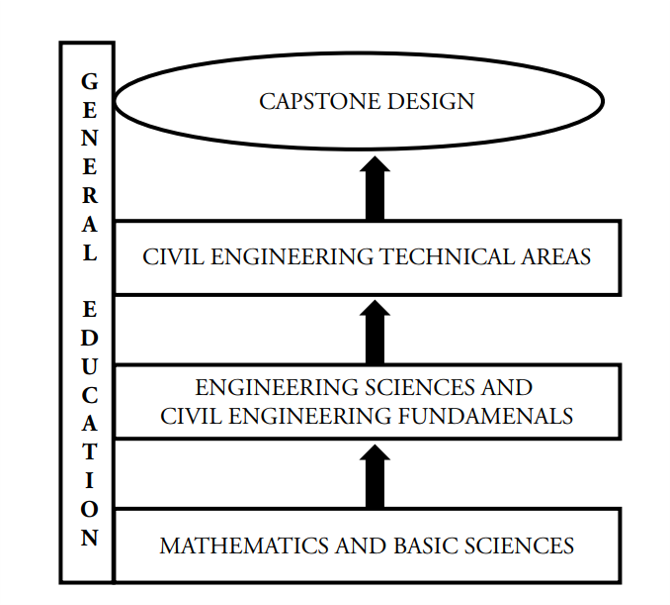
\includegraphics[width=.45\linewidth]{curriculum_structure.png}
			\caption{Curriculum Structure}
		\end{figure}
	\end{frame}

	\begin{frame}{General Education}
		complements the technical content of the curriculum consistent 
		with the program and institution objectives\\
		\bigskip
		\visible<2->{college graduate should have knowledge and skills in areas
		vital to understanding of modern society}
	\end{frame}

	\begin{frame}{Mathematics and Basic Sciences}
		Mathematics courses includes basic calculus courses, differential equations, statistics, 
		and numerical methods. \\
		\bigskip
		Basic sciences requirements can be satisfied by either biology, chemistry,
		or other science courses. 
	\end{frame}

	\begin{frame}{Engineering Sciences}
		Required for most engineering disciplines. Typically includes:
		\begin{itemize}
			\item<2-> \textbf{Statics} - deals with forces and equilibrium, and the concepts derived thereof
			\item<3-> \textbf{Dynamics}  - deals with motion of objects and its relationship with forces
			\item<4-> \textbf{Fluid Mechanics} - studies the movement of fluids in open and enclosed environment
		\end{itemize}		
	\end{frame}

	\begin{frame}{Civil Engineering Fundamentals}
		Courses required for Civil Engineering but are not for most other engineering disciplines.
		Typically includes:
		\begin{itemize}
			\item<2-> \textbf{Engineering Materials} - studies the manufacturing and the properties of 
			materials for engineering applications
			\item<3-> \textbf{Mechanics of Materials}  - studies the effects of forces acting on structural members 
			on the material of the members
			\item<4-> \textbf{Soil Mechanics} - studies the behavior of soil and rocks supporting civil engineering
			structures
			\item<5-> \textbf{Hydrology} - studies and quantifies the circulation and movement of water
		\end{itemize}
	\end{frame}

	\begin{frame}{Allied Courses}
		Includes introductory courses from other engineering disciplines, such as:
		\begin{itemize}
			\item<2-> \textbf{Basic Electric Engineering} - covers electric circuit analysis, tranformers, power supply, etc
			\item<4-> \textbf{Thermodynamics} - studies the conversion among different forms of energy
			\item<4-> \textbf{Computer Programming} - covers either fundamentals of computer programming or tools of
			computing for civil engineers
		\end{itemize}
		
	\end{frame}

	\begin{frame}{Professional Courses}
		Includes courses focused on Civil Engineering technical areas. For Structural Engineering: 
		\begin{itemize}
			\item<2-> \textbf{Structural Theory} - studies further analytical tools for computing 
			the member forces and the deflections of beams, trusses, and frames.
			\item<3-> \textbf{Reinforced Concrete Design} - covers beam design, simple slab design, column design, and simple foundation design using concrete
			and reinforcing steel bars
			\item<4-> \textbf{Steel Structures Design} - deals with design of tension and compression members made of steel
			including their connections (welded, bolted)
		\end{itemize}
	\end{frame}

	\begin{frame}{Capstone Design}
		The culmination of the curriculum which involves a major design experience based on the
		knowledge and skills acquired in earlier courses.
	\end{frame}

%------------------------------------------------



%------------------------------------------------

%\section*{References}
%\SectionPage

%------------------------------------------------

%\begin{frame} % Use [allowframebreaks] to allow automatic splitting across slides if the content is too long
%	\frametitle{References}
%	
%	\begin{thebibliography}{99} % Beamer does not support BibTeX so references must be inserted manually as below, you may need to use multiple columns and/or reduce the font size further if you have many references
%		\footnotesize % Reduce the font size in the bibliography
%		
%		\bibitem[Smith, 2022]{p1}
%			John Smith (2022)
%			\newblock Publication title
%			\newblock \emph{Journal Name} 12(3), 45 -- 678.
%			
%		\bibitem[Kennedy, 2023]{p2}
%			Annabelle Kennedy (2023)
%			\newblock Publication title
%			\newblock \emph{Journal Name} 12(3), 45 -- 678.
%	\end{thebibliography}
%\end{frame}


%----------------------------------------------------------------------------------------
%	CLOSING SLIDE
%----------------------------------------------------------------------------------------

\begin{frame}[plain] % The optional argument 'plain' hides the headline and footline
	\begin{center}
		{\Huge The End}
		
		\bigskip\bigskip % Vertical whitespace
		
		{\LARGE Questions? Comments?}
	\end{center}
\end{frame}

%----------------------------------------------------------------------------------------

\end{document} 